\begin{document}

\section{Sprint 3}

\textbf{Goals for Sprint 3}\\\\
    
    Autonomous
    \begin{itemize}
        \item Use encoders to figure out our position on the field
        \item Move the Foundation and park under the Skybridge during autonomous
    \end{itemize}
    
    Building
    \begin{itemize}
        \item Build new version of the current simple outtake
        \item Design a new, more complex outtake that we won't use for the next league meet.
    \end{itemize}
\vspace{1in}



\meetingnotes{11/11/19 3:00pm - 4:00pm}{Sprint 3 - Meeting}{Josh, Julia, Liana, Michael, Oliver, Ori, Rachel, Sarah}{
    
    Drivetrain motor encoders & We need to have encoders on the drivetrain motors in order to use Road Runner effectively to code our autonomous.\\\\
    
    New temporary outtake & Our LM1 outtake was built less than a day before competition and was made of cardboard. It was very simple and just flipped the Stones onto the Foundation. We will make a similar version out of something more sturdy than cardboard for LM2, and will probably have a claw design after LM2.\\\\
    
    New outtake design and claw & \\\\
    
    Autonomous & We plan to have as close to a full autonomous as we can by LM2 and will dedicate the majority of our practice time to working on the code.
}



\practicenotes{11/11/19 4:00pm - 7:00pm}{Sprint 3 - Practice}{Josh, Julia, Liana, Michael, Oliver, Ori, Rachel, Sarah}{

    Programming\\\\
    \textit{Tuning: }Josh and Michael worked on getting encoder, localization, and PID values to be accurate.\\\\
    Written by: Rachel
    
}



\practicenotes{11/13/19 6:30pm - 9:00pm}{Sprint 3 - Practice}{Dominik, Josh, Julia, Liana, Michael, Oliver, Ori, Rachel, Sarah}{
    
    Building\\\\
    \textit{Adjusting: }We need to take apart a lot of the chassis in order to rotate some of the drivetrain motors so that we can plug encoders in, which we need for autonomous.\\\\
    Written by: Rachel
    \newBox
    
    CAD and Design\\\\
    \textit{Phone Mount and Intake: }Ori is working on CADing a new phone mount that isn't angled down as much so that the phone can see the Stones and Navigation Targets from further away. Oliver is editing his CAD model of the intake to make the mount for the servo stronger (we broke it at LM1) and to make sure the belt is tensioned. We will reprint components of the intake as necessary.\\\\
    Written by: Rachel
    \newBox
    
    Programming\\\\
    \textit{Vision: }Josh is working on getting test code from last year to work on vision in autonomous that will be used to find the Foundation in case our alliance partner moves it during autonomous.\\\\
    Written by: Rachel
    \newBox
    
    Logistics\\\\
    \textit{Outreach: }I sent some emails to the feeder schools to Wilson to check in and see if any of them had science fairs or other events that we could participate in. I also sent an email to the local library to ask if we could do a robot showing there. Additionally, there was a rough draft email created for the students who had expressed interest in the Robotics Club at the 8th Grade Family Night that had occurred previously at our high school.\\\\
    Written by: Sarah
}



\practicenotes{11/15/19 3:30pm - 9:00pm}{Sprint 3 - Practice}{Dominik, Josh, Julia, Liana, Michael, Oliver, Ori, Rachel, Sarah}{

    CAD and Design\\\\
    \textit{Outtake Design: }Oliver is working on a CAD model for the new outtake, which we are not planning on having for League Meet 2.\\\\
    Written by: Rachel
    \newBox
    
    Programming\\\\
    \textit{Tuning: }Michael ran tests to tune track width, and edited drive constants based on that in autonomous. We also ran several tests by running Drive Velocity PID Tuner (calculates a scalar for voltage to acceleration), Straight Test (tests if Drive Velocity PID Tuner worked), Track Width Tuner (finds the distance between the left and right wheels), Turn Test (determines whether Track Width Tuner was accurate or not), Spline Test (makes the robot go in a complicated path, and calculates error. Is used to test all previous tests), Follower PID Tuner (tunes the PID to better follow paths). Josh worked on TeleOp code.\\\\
    Written by: Michael
    \newBox
    
    Driver practice\\\\
    \textit{Driver-Centric: }Oliver, Julia, and Dominik all spent some time driving a driver-centric mecanum-wheeled robot, that drives similar to how ours would if we chose to use a driver-centric op-mode.\\\\
    Written by: Rachel
    \newBox
    
    Logistics\\\\
    \textit{Outreach: }Sarah continued to work on setting up outreach and connect with other locations. She was put in contact with the science fair managers of both Markham Elementary School and Stephenson Elementary School. She also got in contact with some people at the local library to plan a robot showing where we would enlighten them with our knowledge. The club was also given a contact for a retirement center in Beaverton which was looking forward to having us come over and show the residents the robot.\\\\
    Written by: Sarah
}



\practicenotes{11/17/19 12:00pm - 7:30pm}{Sprint 3 - Practice}{Liana, Michael, Oliver, Sarah}{

    CAD and Design\\\\
    \textit{Outtake Design: }Oliver continued to work on CADing the outtake for the robot.\\\\
    Written by: Sarah
    \newBox
    
    Programming\\\\
    \textit{Testing and Wiring: } Michael, with help from our mentor, Jaren, worked on the localization for the robot. They messed with some values to see which ones would turn however much they wanted. Unfortunately, for some reason, the odometry pod encoders weren't working. We found out that the problem was that the e4ts had been plugged in backwards into the levellers. Fortunately, after that changed, everything worked out.\\\\
    Written by: Sarah
}


\practicenotes{11/18/19 3:30pm - 9:00pm}{Sprint 3 - Practice}{Julia, Liana, Michael, Oliver, Sarah}{

    CAD and Design\\\\
    \textit{Intake: }Oliver is currently working on completing the second intake pod for the robot.\\\\
    Written by: Sarah
    \newBox
    
    Programming\\\\
    \textit{Debugging: }Michael came across some errors in the code where the robot would have delayed response in stopping. Additionally, Michael was having some problems with the robot code acknowledging the gyro.\\\\
    Written by: Sarah
}



\practicenotes{11/20/19 6:00pm - 9:00pm}{Sprint 3 - Practice}{Dominik, Josh, Julia, Michael, Rachel}{

    Programming\\\\
    \textit{Localization: }We are switching to a two wheel localizer, because it lets us use the gyro for heading. This new localizer should fix most of our problems with an inaccurate heading.\\\\
    Written by: Rachel
    \newBox
    
    CAD and Design\\\\
    \textit{Outtake Design: }Oliver is working on a CAD model of our new outtake, which is similar to what we had for LM0, but we are shifting the location of the belt and only having one slide going up on each side instead of two (for now).
    \\\\
    %CAD of outtake final
    Written by: Rachel
    \newBox
    
    Building\\\\
    \textit{Outtake: }Julia and Dominik are building a new flipper outtake that we will plan on using unless Oliver completes his intake. The flipper is very similar to what we had at LM1 but is built from a stronger material and will work better.\\\\
    Written by: Rachel
}



\practicenotes{11/22/19 3:30pm - 11:00pm}{Sprint 3 - Practice}{Julia, Liana, Michael, Oliver, Rachel, Sarah}{
    Building\\\\
    \begin{wrapfigure}{l}{.41\textwidth}
        \begin{center}
            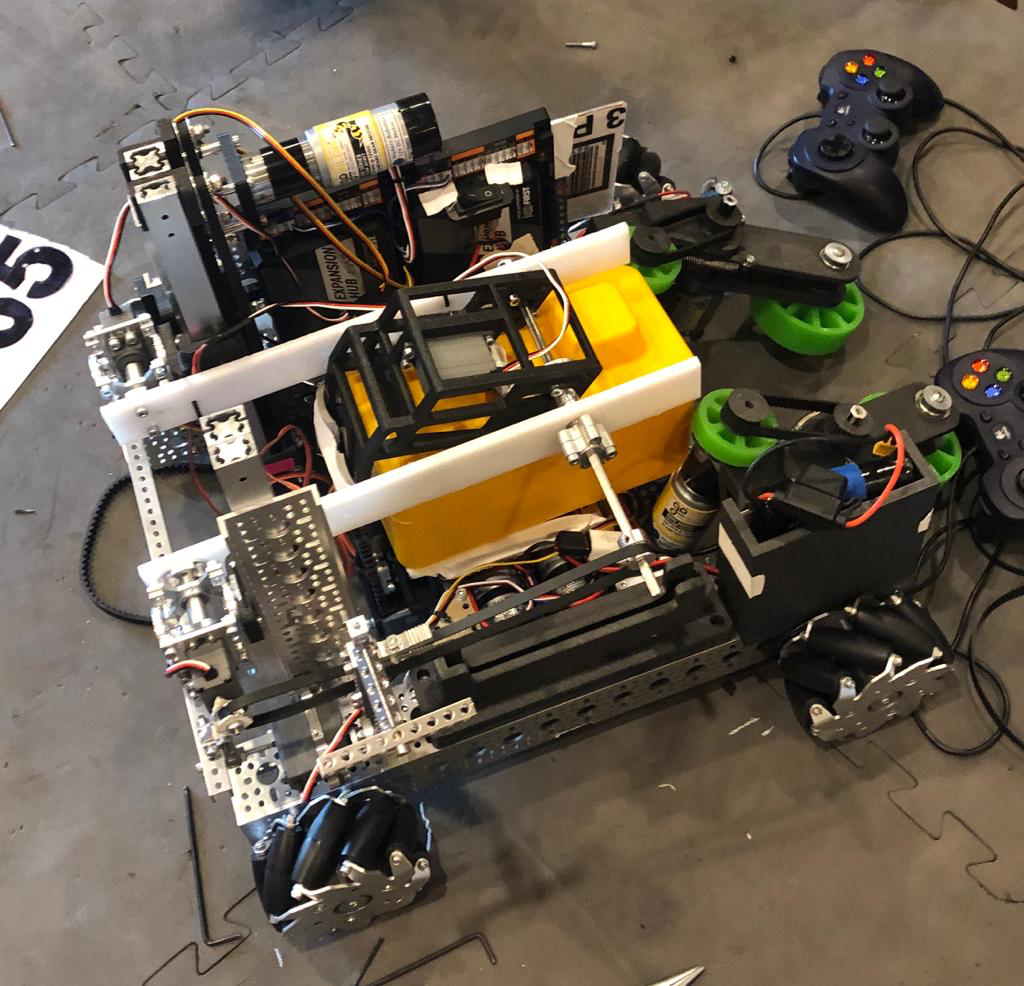
\includegraphics[width=.4\textwidth]{Images2/11-22robotstone.png}
        \end{center}
    \end{wrapfigure}
    \textit{Intake and Outtake: }We finished printing the servo blocks, battery mounts, and some other things for the outtake that Oliver designed. We replaced the intake pods (the new ones are sturdier) and attached stronger springs. We mounted the servo to the new claw that we 3D printed and the pieces to grip the Stone. Oliver, Liana, and Julia worked on assembling the slides and arm for the outtake and connecting all the components and wires.
    Michael managed all of the wires so they wouldn't get in the way of the intake or the outtake.\\\\\\
    Written by: Julia
    %CAD of claw with Stone
    %CAD of robot morning of meet before we took the outtake off
    \newBox
    
    Programming\\\\
     \begin{wrapfigure}{r}{.41\textwidth}
        \begin{center}
            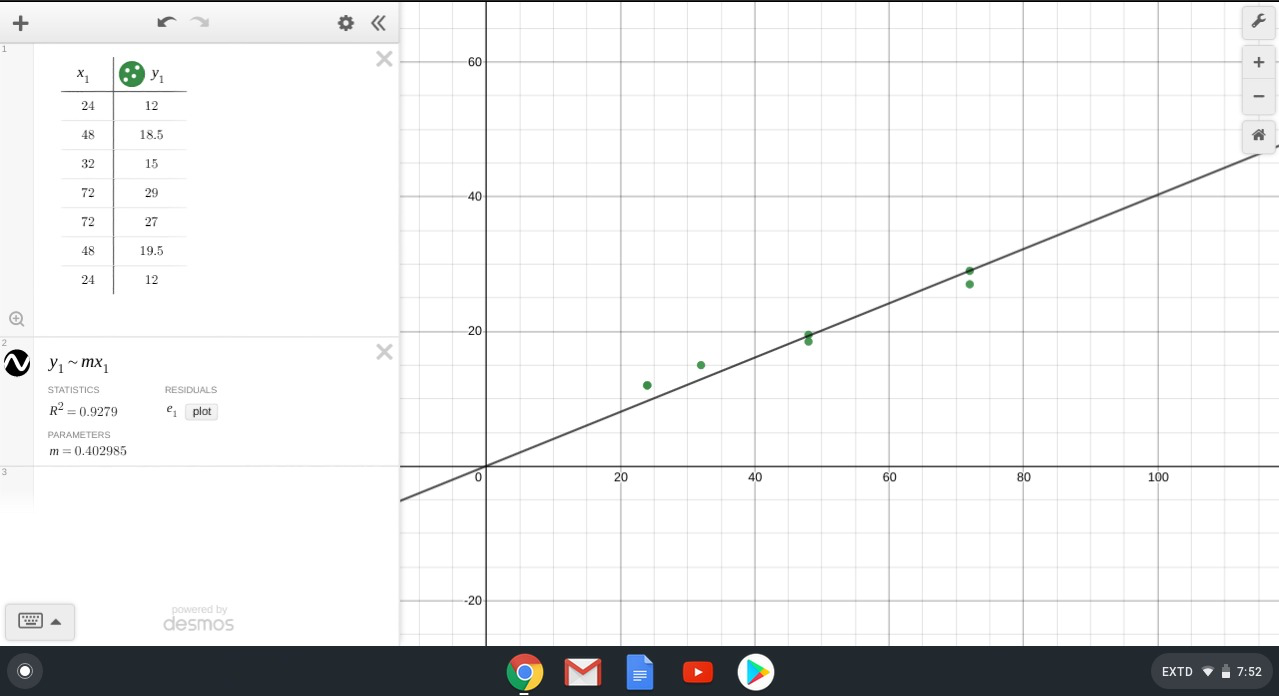
\includegraphics[width=.4\textwidth]{Images2/11-22graph1.png}
            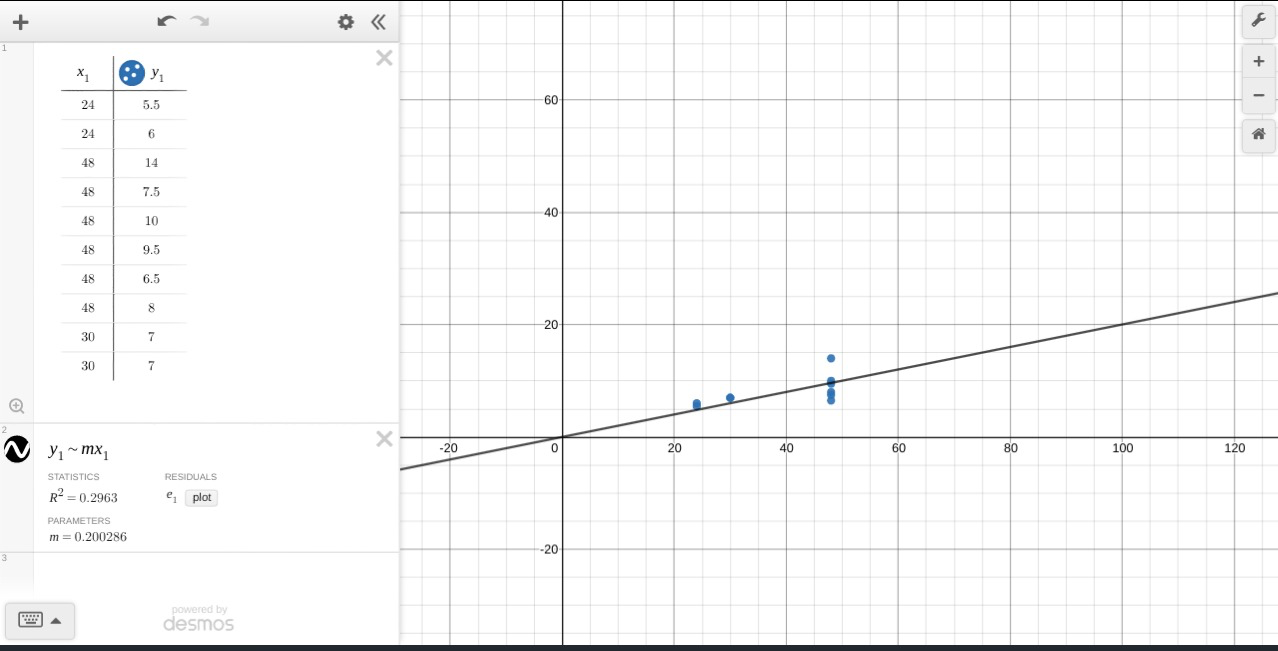
\includegraphics[width=.4\textwidth]{Images2/11-22graph2.png}
        \end{center}
    \end{wrapfigure}
    \textit{Vuforia and Tuning:} Michael continued to work on the autonomous code. He got Vuforia to recognize the Skystones. We are testing the encoder inputs and writing code to compensate for some errors that we noticed were consistently happening by multiplying the input from the odometry pods by a constant that we determined by interpolating error in drive distances.\\\\
    \textit{Autonomous: }We tested the servos to pull the \\Foundation servos and they work well. Since\\ we pull the Foundation by driving sideways, \\we realized that the ideal spot to hold the \\Foundation is actually not in the middle but\\ further back.\\\\
    Written by: Rachel
}



\img{Images2/11-22foundation.png}{Testing moving the foundation in autonomous}{.75}
\xvspace



\meetingnotes{11/23/19 1:00pm - 5:00pm}{League Meet 2}{Dominik, Julia, Liana Michael, Oliver, Rachel, Sarah}{

    Overview & We ended up having to revert to our old outtake system the morning of the League Meet, so we were only able to flip the Stones onto the Foundation and not stack them. We had an autonomous code to move the Foundation that almost worked, which we can fine-tune and get to work next time. Our code to just park under the Foundation was good and we could park either close to the wall or close to the middle of the Skybridge depending on our alliance partner. After the meet, we were in 7th out of the 10 teams combining scored from both meets. Two of the usual drive team members were gone so the driving wasn't as good as it couldn't been.\\\\
    
    What went well & \begin{itemize}
        \item Autonomous to park under the Skybridge in either position
        \item Our intake worked well enough and could pick up the Stones from several different angles
    \end{itemize}\\\\
    
    What needs improvement & \begin{itemize}
        \item Driver practice
        \item Autonomous to move Foundation
        \item Stronger springs on intake
        \item Outtake to stack Stones.
    \end{itemize}
}



\practicenotes{11/25/19 6:00pm - 2:00am}{Sprint 3 - Practice}{Michael, Oliver}{

    Building\\\\
    \textit{Wiring: }I replaced a broken odometry pod broken wire and plugged the other one into the correct port.\\\\
    Written by: Michael
    \newBox
    
    CAD and Design\\\\
    \textit{Design: }Oliver and I decided that we needed a better mechanism to transfer the Stone from the intake to the outtake. Oliver will design a holder for the Stone that will sit right above the chassis and keep it in position for the outtake. We also decided to rotate the slides on our outtake to allow for more expansion with additional slides, as well as a more forgiving claw. There was talk of altering the intake, but it was dismissed because we have more important things to focus on.\\\\
    Written by: Michael
    
    %add cad of the thing
    \newBox
    Programming\\\\
    \textit{Tuning: }I started tuning the PID coefficients for translational movement, and managed to get an accurate distance, however there was significant error in where the bot was and where it should have been while it was driving. My next step will be to repeat this process with the heading PID coefficients. If those go well, I should be able to run a spline test and get an accurate result. If not, more tuning will be required.\\\\
    Written by: Michael
}



\practicenotes{11/28/19 1:00pm - 1:00am}{Sprint 3 - Practice}{Michael}{

    Programming\\\\
    \textit{Autonomous: }I messed around with Vuforia, and couldn't get it to work with the lighting (or something). I then spent some time reading documentation on Road Runner PID control, as well as some time tuning translational, heading, and velocity PID coefficients. At around 10:30 I was getting a weird dashboard error, that prevented me from doing any more tuning, so I started writing up an auto that would grab a Skystone with the intake.\\\\
    \textit{Organization: }Testing will need to get done. I also moved the code I had been working on that was on Jaren's repository into a new repository on my account. This new repository at the moment has three things: a clean Road Runner project to duplicate anytime we need a clean slate, a project full of various Vuforia tests, and our main Skystone project, that houses all of our code for this years challenge. This new structure should help keep us organized, and keep everything we need in an easily accessible, unified place.\\\\
    Written by: Michael
}



\practicenotes{11/29/19 1:15am - 3:30am}{Sprint 3 - Practice}{Michael}{

    Programming\\\\
    \textit{Tele-op: }I got bored after a few minutes so I started work on writing some tele-ops. I created a basic mecanum drive, where the left stick controls movement, and the right stick controls rotation. I then made a driver centric mecanum drive, which basically keeps track of what angle the robot is at, and uses polar coordinates to make it so pushing up on the left joystick causes the robot to move upwards (away from the driver) no matter what orientation it is in to start with. Finally, I started work on a absolute rotation driver centric mecanum drive, which is essentially a driver centric mecanum drive, but instead of the right stick rotating the bot, the bot rotates to whatever position the tight stick is at.\\\\
    Written by: Michael
}



\practicenotes{11/29/19 1:00pm - 8:00pm}{Sprint 3 - Practice}{Michael}{

    Programming\\\\
    \textit{Understanding Roadrunner: }I played around with some more PID tuning stuff. I had a big revelation on how PID works as well, which really helped me understand everything a lot better. Not a lot of quantifiable progress made today, but I understand things a lot better now.\\\\
    Written by: Michael
}



\practicenotes{11/30/19 11:00am - 4:00pm}{Sprint 3 - Practice}{Michael}{

    Programming\\\\
    \textit{Tuning: }I finished tuning velocity PID coefficients, so it should be able to correct itself if its velocity gets off course. I then tuned the track-width (lateral distance between wheels), and then ran some tests. The bot does very well with forward and backwards movement, as well as turning, however lateral movement can get a little wonky. I have yet to tune the position and heading PID, and that should solve most of our problems. We did have a motor that performs significantly worse than the other for no apparent reason. We have ordered a new one, and it should come Monday. Replacing this motor should help with the error in the lateral movement.\\\\
    Written by: Michael
}



\practicenotes{12/1/19 10:00am - 12:00am}{Sprint 3 - Practice}{Josh, Liana, Michael}{

    Building\\\\
    \textit{3D-Printing: }Michael broke one of the arms of the intake, so we need to print a new one. Liana glued it back together for temporary use. She also soldered a broken wire back together. We may or may not print it depending on how much extra time we have to print.\\\\
    Written by: Michael
    \newBox
    
    Programming\\\\
    \textit{Tuning: }Josh starting thinking about our plan for autonomous, and what different op-modes we want to be able to run, and what they will do. Michael fixed the absolute rotation tele-op code, and tuned the heading PID. He then spent most of the rest of practice trying to tune the translational PID, and got values that will work for now. He then wrote a quick and dirty script that would grab a Skystone, however he couldn't get Vuforia to get the position of the stone after moving the robot, however he did get Vuforia to work on its own. He still doesn't think he is using Roadrunner correctly, but he did manage to scrape together an auto that will grab one Skystone.\\\\
    Written by: Michael
}
\end{document}